\chapter{Opis projektnog zadatka}

		
		Cilj ovog projekta je timskim radom i korištenjem našeg znanja
		oblikovanja programske potpore razviti web aplikaciju "FringillaSport".
		Cilj aplikacije "FringillaSport" je omogućiti jednostavnije povezivanje sportaša, 
		trenera i iznajmljivača sportskih prostora te taj proces pojednostavniti i ubrzati.
		
		Aplikaciju mogu koristiti i registrirani i neregistrirani korisnici. 
		Registrirani korisnici mogu biti:
		
		\begin{packed_item}
			\item{Administrator}
			\item{Iznajmljivač}
			\item{Trener}
			\item{Sportaš}
		\end{packed_item}
	
		Pri registriranju korisnik bira ulogu Sportaša, Trenera ili Iznajmljivača. Za registraciju Sportaša, Trenera i Iznajmljivača
		su potrebni sljedeći podaci:
		
		\begin{packed_item}
			\item{ime}
			\item{prezime}
			\item{email}
			\item{koriničko ime}
			\item{zaporku}
		\end{packed_item}
	
	Za registraciju Trenera potrebno je još priložiti i službenu dokumentaciju koja potvrđuje da je ta osoba službeni trener za neke sportove 
	(takvu prijavu odobrava administrator koji provjerava vjerodostojnost informacija). 
	
	Mogućnosti korisnika:
	
	\begin{packed_item}
		\item{Neregistrirani korisnik:
			\begin{packed_item}
				\item{Pristup stranici te pristup tražilici sportskih okupljanja/treninga. 
					(Korisnik ima samo pregled, ne može se prijaviti na sportsko okupljanje/trening.)
				}
			\end{packed_item}
		}
	
		\item{Sportaš:
			\begin{packed_item}
				\item{Pristup tražilici sportskih okupljanja/treninga.}
				\item{Prijava za pojedino sportsko okupljanje/trening unutar tražilice sportskih okupljanja/treninga.
				}
				\item{Vidljivost svih prijavljenih događaja u vlastitom kalendaru sportskih okupljanja/treninga.
				}
				\item{Dobivanje preporuke za odabir sporta u kojem bi imao najveće mogućnosti ostvariti izvrsne
					rezultate na natjecanjima. Preporuka se temelji na visini, težini, broju godina i
					ostalih osobnih podataka.}
				\item{Može zatražiti ulogu trenera ako dobije službeni certifikat.
				}
			\end{packed_item}}
	
			\item{Iznajmljivač:
			\begin{packed_item}
				\item{Može imati odvojeni račun trenera/sportaša.}
				\item{Može u uređivaču sportskih objekata dodati svoj sportski objekt navodeći lokaciju, 
					tip sportova koji se mogu u objektu održavati, cijenu po satu, termine dostupne za rezervaciju i 
					dokumentaciju koja potvrđuje da je on vlasnik. (Takvu prijavu administrator provjerava i 
					potvrđuje ako je sve ispravno.)}
				\item{U svom kalendaru može vidjeti trenutno odobrene termine za iznajmljivanje i nove termine za koje
					je netko od korisnika zatražio iznajmljivanje te takve termine odobriti ili odbaciti.
				}
			\end{packed_item}}
		
		\item{Trener:
			\begin{packed_item}
				\item{Može naknadno prijaviti dodatnu službenu dokumentaciju. (Za neki drugi sport ili slično.)
				}
				\item{Mogućnost organiziranja i naplaćivanja treninga u sportovima za koje ima potvrđenu dokumentaciju.
					Trening se može organizirati u uređivaču treninga po istom principu kao što se organizira sportsko
					okupljanje.}
				\item{Nasljeđuje prava sportaša te može organizirati i sportska okupljanja za ostale sportove.
				}
				\item{Uz kalendar sportskih okupljanja na kojima on prisustvuje izvan profesionalnih
					treninga, ima i pristup kalendaru svih svojih termina treninga te podatke o njima.
					 ime}
			\end{packed_item}}
		
		\item{Administrator:
			\begin{packed_item}
				\item{Upravlja sustavom.}
				\item{Odobrava i provjerava istinitost podataka iznajmljivača sportskih objekata i trenera koji se 
					žele registrirati u aplikaciju.}
				\item{Može brisati ili dodavati druge korisnike te im mijenjati uloge. (Brisanjem određenog korisnika, 
					brišu se sve njegove prijave na sportska okupljanja i/ili svi termini treninga kreirani od tog korisnika
					ili/i svi sportski objekti kreirani.)
				}
			\end{packed_item}}
	\end{packed_item}
		
		
		\section{Postojeća slična rješenja}
		
		Aplikacija slična aplikaciji koju mi razvijamo je \clickablefootnotelink{playeasy}{https://www.playeasy.com/}. Playeasy je aplikacija dizajnirana za pretraživanje i iznajmljivanje sportskih objekata ili površina. Pretraživanje je puno detaljnije za razliku od aplikacije koju mi razvijamo s mogućnostima sužavanja rezultata na temelju sporta, tipa prostora (dvorana, auditorij, teretana...), tipa površine (beton, drvo, zemlja...) i drugih.
		
		\begin{figure}[H]
			
\includegraphics[scale=0.6]{slike/playeasy-pretrazivanje.PNG} %veličina slike u odnosu na originalnu datoteku i pozicija slike
			\centering
			\caption{playeasy - Pretraživanje}
			\label{fig:promjene}
		\end{figure}
		
		Nakon pretraživanja se otvara popis svih dostupnih objekata i površina, te karta s njihovim lokacijama.
		
		\begin{figure}[H]
			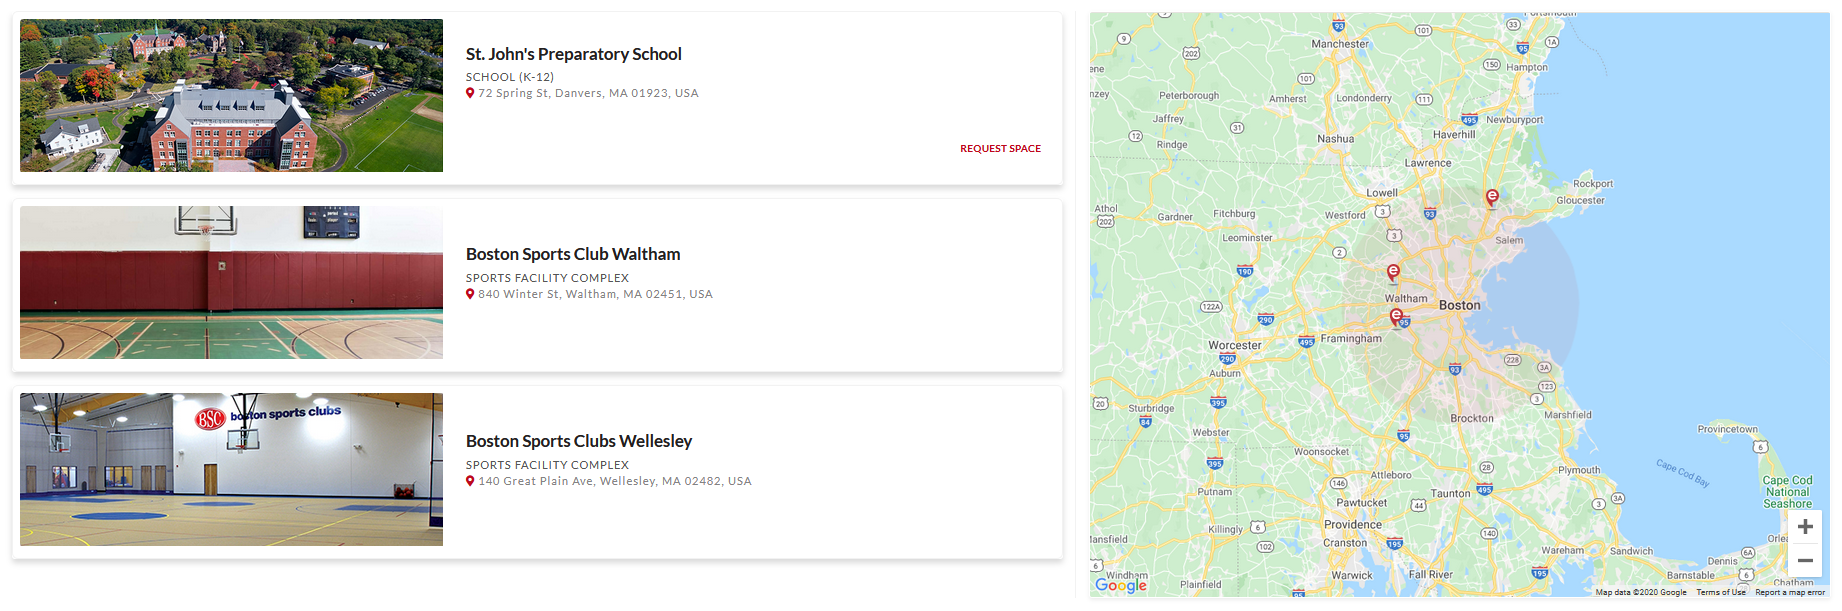
\includegraphics[width=1\linewidth]{slike/playeasy-prikaz.PNG}
			\centering
			\caption{playeasy - Prikaz dostupnih sportskih objekata i površina}
			\label{fig:promjene}
		\end{figure}
		
		Najveća razlika između naše aplikacije i playeasy je što playeasy povezuje samo organizatore sportskih aktivnosti i iznajmljivače, a naša aplikacija povezuje organizatore s iznajmljivačima i sportašima.
		
		Druga slična aplikacija je
		\clickablefootnotelink{teamsnap}{https://www.teamsnap.com/}. Ova aplikacija se fokusira na povezivanje trenera i igrača, te olakšavanje komunikacije između njih. Nema mogućnosti iznajmljivanja sportskih objekata ili površina. Aplikacija sadrži mogućnosti potvrđivanja može li netko doći na trening, grupni chat između članova sportskih ekipa, plaćanje treninga i slične mogućnosti.
		
		\begin{figure}[H]
			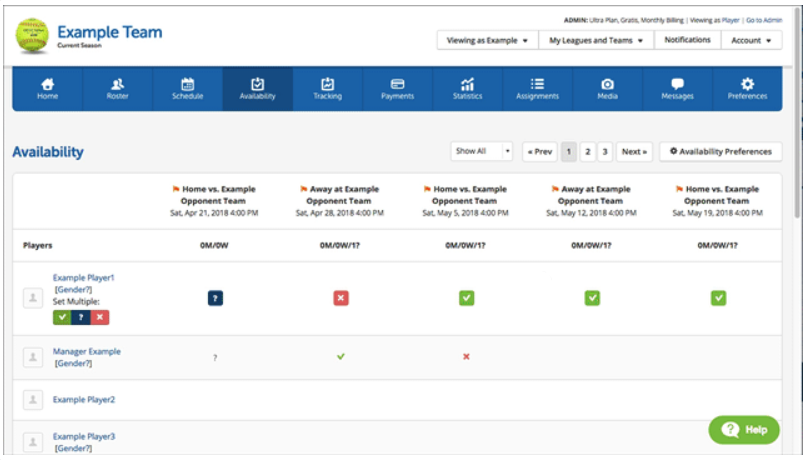
\includegraphics[width=1\linewidth]{slike/teamsnap-dostup.PNG}
			\centering
			\caption{teamsnap - Dostupnost igrača za pojedine sportske događaje}
			\label{fig:promjene}
		\end{figure}
		
		Ostale aplikacije slične našoj su \clickablefootnotelink{uniquevenues}{https://www.uniquevenues.com/} i \clickablefootnotelink{SchoolHire}{https://schoolhire.co.uk/}. Obje ove aplikacije se fokusiraju na iznajmljivanje sportskih površina ili objekata poput aplikacije playeasy, te nemaju mogućnost organiziranja sportskih okupljanja ili treninga.
		
		\section{Moguće nadogradnje projektnog zadatka}
		
		
		Moguća nadogradnja ovog projekta bi bila mogućnost stvaranja sportskih timova. Članovi jednog tima bi mogli međusobno komunicirati, organizirati se i prijavljivati na sportske aktivnosti, te slati upute drugim timovima žele li s njima igrati.
		
		Druga mogućnost bi bila organizacija natjecanja, na koja bi se mogli prijavljivati pojedinci ili timovi ovisno o sportu. Za natjecanje bi se mogao definirati raspored koji bi svi mogli pregledavati, a organizator uređivati.
		
		Još jedna nadogradnja bi mogla biti mogućnost ocjenjivanja trenera, sportskih objekata i površina. Svatko tko je prisustvovao treningu kod nekog trenera ili sportskoj aktivnosti u nekom sportskom objektu ili površini bi mogao ostaviti kratki komentar i ocjenu o tom treneru, sportskom objektu ili površini. 

\iffalse	% zakomentirani primjeri iz latexa, kasnije ukloniti
	
		\section{Primjeri u \LaTeX u}
		
		\textit{Ovo potpoglavlje izbrisati.}\\

		U nastavku se nalaze različiti primjeri kako koristiti osnovne funkcionalnosti \LaTeX a koje su potrebne za izradu dokumentacije. Za dodatnu pomoć obratiti se asistentu na projektu ili potražiti upute na sljedećim web sjedištima:
		\begin{itemize}
			\item Upute za izradu diplomskog rada u \LaTeX u - \url{https://www.fer.unizg.hr/_download/repository/LaTeX-upute.pdf}
			\item \LaTeX\ projekt - \url{https://www.latex-project.org/help/}
			\item StackExchange za Tex - \url{https://tex.stackexchange.com/}\\
		
		\end{itemize} 	


		
		\noindent \underbar{podcrtani tekst}, \textbf{podebljani tekst}, 	\textit{nagnuti tekst}\\
		\noindent \normalsize primjer \large primjer \Large primjer \LARGE {primjer} \huge {primjer} \Huge primjer \normalsize
				
		\begin{packed_item}
			
			\item  primjer
			\item  primjer
			\item  primjer
			\item[] \begin{packed_enum}
				\item primjer
				\item[] \begin{packed_enum}
					\item[1.a] primjer
					\item[b] primjer
				\end{packed_enum}
				\item primjer
			\end{packed_enum}
			
		\end{packed_item}
		
		\noindent primjer url-a: \url{https://www.fer.unizg.hr/predmet/proinz/projekt}
		
		\noindent posebni znakovi: \# \$ \% \& \{ \} \_ 
		$|$ $<$ $>$ 
		\^{} 
		\~{} 
		$\backslash$ 
		
		\begin{longtabu} to \textwidth {|X[8, l]|X[8, l]|X[16, l]|} %definicija širine tablice, širine stupaca i poravnanje
			
			%definicija naslova tablice
			\hline \multicolumn{3}{|c|}{\textbf{naslov unutar tablice}}	 \\[3pt] \hline
			\endfirsthead
			
			%definicija naslova tablice prilikom prijeloma
			\hline \multicolumn{3}{|c|}{\textbf{naslov unutar tablice}}	 \\[3pt] \hline
			\endhead
			
			\hline 
			\endlastfoot
			
			\rowcolor{LightGreen}IDKorisnik & INT	&  	Lorem ipsum dolor sit amet, consectetur adipiscing elit, sed do eiusmod  	\\ \hline
			korisnickoIme	& VARCHAR &   	\\ \hline 
			email & VARCHAR &   \\ \hline 
			ime & VARCHAR	&  		\\ \hline 
			\cellcolor{LightBlue} primjer	& VARCHAR &   	\\ \hline 
			
		\end{longtabu}
		

		\begin{table}[H]
			
			\begin{longtabu} to \textwidth {|X[8, l]|X[8, l]|X[16, l]|} 
				
				\hline 
				\endfirsthead
				
				\hline 
				\endhead
				
				\hline 
				\endlastfoot
				
				\rowcolor{LightGreen}IDKorisnik & INT	&  	Lorem ipsum dolor sit amet, consectetur adipiscing elit, sed do eiusmod  	\\ \hline
				korisnickoIme	& VARCHAR &   	\\ \hline 
				email & VARCHAR &   \\ \hline 
				ime & VARCHAR	&  		\\ \hline 
				\cellcolor{LightBlue} primjer	& VARCHAR &   	\\ \hline 
				
				
			\end{longtabu}
	
			\caption{\label{tab:referencatablica} Naslov ispod tablice.}
		\end{table}
		
		
		%unos slike
		\begin{figure}[H]
			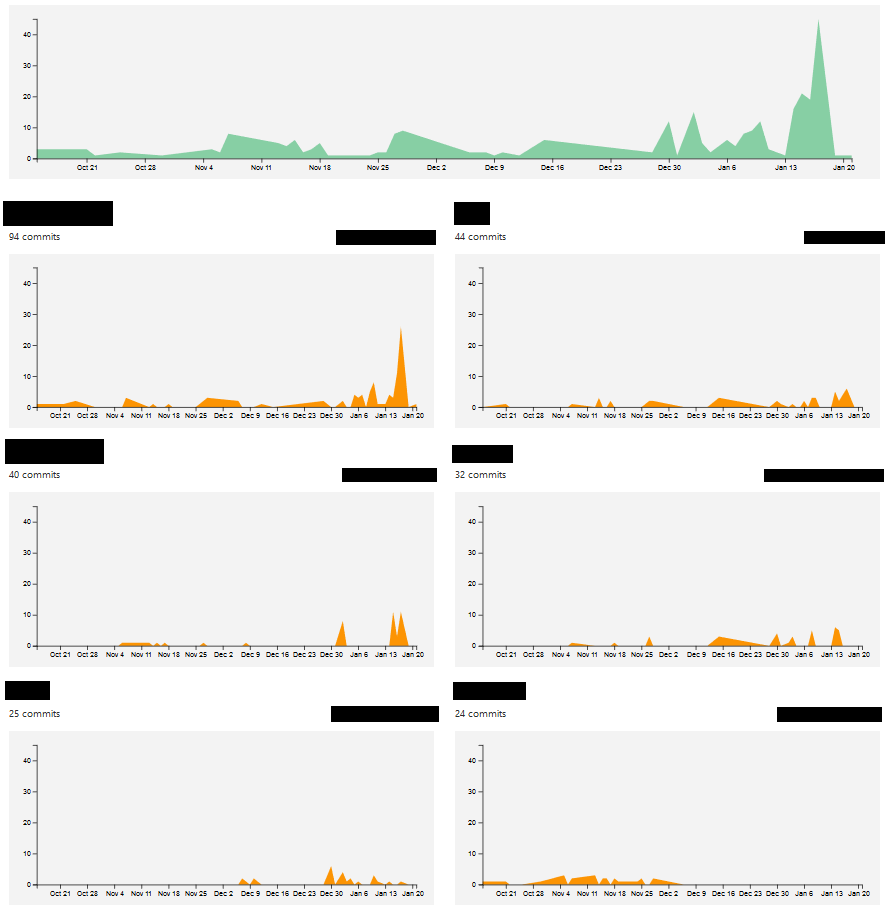
\includegraphics[scale=0.4]{slike/aktivnost.PNG} %veličina slike u odnosu na originalnu datoteku i pozicija slike
			\centering
			\caption{Primjer slike s potpisom}
			\label{fig:promjene}
		\end{figure}
		
		\begin{figure}[H]
			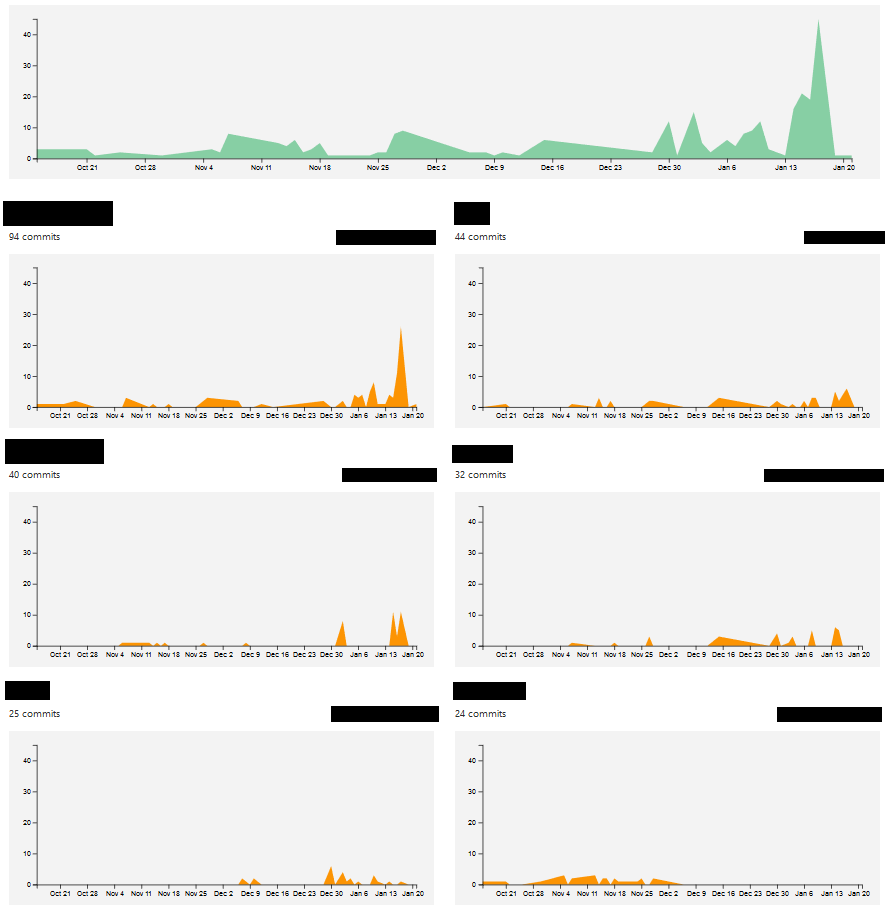
\includegraphics[width=.9\linewidth]{slike/aktivnost.PNG} %veličina u odnosu na širinu linije
			\caption{Primjer slike s potpisom 2}
			\label{fig:promjene2} %label mora biti drugaciji za svaku sliku
		\end{figure}
		
		Referenciranje slike \ref{fig:promjene2} u tekstu.
		
		\eject
\fi	